\documentclass[11pt,a4paper]{article}
\usepackage[utf8]{inputenc}
\usepackage[T1]{fontenc}
\usepackage[italian]{babel}
\usepackage{lmodern}
\usepackage[a4paper,margin=2.3cm]{geometry}
\usepackage{graphicx}
\usepackage{booktabs}
\usepackage{longtable}
\usepackage{tabularx}
\usepackage{array}
\usepackage{float}
\usepackage{amsmath}
\usepackage{siunitx}
\usepackage{enumitem}
\usepackage{xcolor}
\usepackage{hyperref}
\usepackage{xurl}
\usepackage{microtype}
\usepackage{csquotes}
\usepackage[backend=biber,style=numeric,sorting=nyt]{biblatex}
\addbibresource{bibliography.bib}
\hypersetup{colorlinks=true,linkcolor=blue!55!black,citecolor=blue!55!black,urlcolor=blue!55!black,pdftitle={Biblioteche Fantasma},pdfauthor={Progetto universitario di Open Data Management}}
\setlength{\parskip}{0.45em}
\setlength{\parindent}{0pt}
\setcounter{tocdepth}{2}
\newcommand{\bfproj}{\textit{Biblioteche Fantasma}}
\newcommand{\sourceNote}{Elaborazione su snapshot ICCU 08/09/2026 e ISTAT POSAS 2019--2025, salvo diversa indicazione.}
\newcommand{\pct}[1]{\num[round-mode=places,round-precision=2]{#1}\%}
\title{\textbf{BIBLIOTECHE FANTASMA}\\[0.3em]\large Analisi, integrazione e modellazione semantica delle biblioteche italiane non pienamente operative}
\author{Progetto universitario di Open Data Management}
\date{Anno accademico 2025/2026 -- versione finale 8 settembre 2026}

\begin{document}
\maketitle
\begin{abstract}
Il progetto sviluppa una pipeline completa di Open Data Management a partire da dati reali dell'Anagrafe delle Biblioteche Italiane (ICCU) e della popolazione residente ISTAT POSAS 2019/2025. Le prime due fasi hanno prodotto dati puliti e integrati, metadati, un'ontologia che riusa Cultural-ON, RDF, SHACL, interlinking e query SPARQL. La terza fase, oggetto principale di questa relazione, realizza l'analisi statistica, la data visualization, l'interpretazione delle Research Questions e la chiusura riproducibile del repository. Il master ICCU contiene 19.611 record; il perimetro analitico delle biblioteche problematiche comprende 2.497 casi su 18.956 biblioteche, pari al 13,17\%. La relazione tra variazione demografica comunale 2019--2025 e quota di biblioteche problematiche è debole (Pearson $r=-0{,}106$, Spearman $\rho=-0{,}067$, $N=6.659$). La rete delle confluenze comprende 1.412 archi validati. L'interlinking raggiunge il 100\% verso ICCU per le biblioteche e il 99,9620\% verso Linked ISPRA per i comuni. I risultati vengono interpretati in modo conservativo: i missing non sono trattati come zeri, la correlazione non è causalità e ``Biblioteche Fantasma'' è un'etichetta narrativa, non una categoria ufficiale ICCU.
\end{abstract}
\tableofcontents
\clearpage

\section{Introduzione}
\subsection{Contesto}
Gli Open Data non consistono soltanto nella disponibilità di file scaricabili: richiedono qualità, licenze chiare, formati aperti, metadati, identificatori, interoperabilità e, ai livelli più avanzati, collegamenti verso risorse esterne. Il corso di Open Data Management affronta esplicitamente questo percorso, includendo RDF, RDFS/OWL, triplestore e SPARQL. Il modello a cinque stelle fornisce una sintesi progressiva: dalla pubblicazione con licenza aperta fino ai Linked Open Data collegati al Web of Data \cite{five_star,heathbizer}.

\subsection{Motivazione}
Il dominio bibliotecario è adatto a un progetto di integrazione perché combina un registro nazionale, identificatori istituzionali, coordinate, classificazioni, patrimonio, fondi speciali e dati territoriali. Lo snapshot ICCU registra inoltre stati eterogenei: cessazione, chiusura temporanea, inagibilità, sospensione per sisma, confluenza e altri casi. Queste etichette non possono essere appiattite in una singola nozione di ``biblioteca chiusa''.

\bfproj{} è quindi una cornice narrativa per studiare le biblioteche che, nello snapshot, presentano condizioni di non piena operatività o trasformazioni particolari. Non è un termine ICCU e non viene introdotto come classe ontologica ufficiale.

\subsection{Obiettivi}
Gli obiettivi sono: (i) documentare una pipeline riproducibile di selezione, cleaning, integrazione e pubblicazione; (ii) costruire un dataset analitico comunale; (iii) modellare il dominio in RDF riusando vocabolari esistenti; (iv) collegare biblioteche e comuni a risorse esterne; (v) rispondere con dati reali a domande territoriali, demografiche, patrimoniali e di rete; (vi) produrre visualizzazioni leggibili e una data story metodologicamente prudente.

\subsection{Research Questions}
\begin{enumerate}[label=RQ\arabic*.]
\item Dove sono distribuite le biblioteche caratterizzate da stati di non piena operatività?
\item Quali stati sono più frequenti e come variano tra regioni, province e comuni?
\item Quali tipologie funzionali/amministrative sono maggiormente associate ai diversi stati?
\item Esiste un'associazione tra variazione demografica comunale 2019--2025 e quota di biblioteche con cessazione o interruzione del servizio?
\item Quale patrimonio e quali fondi speciali risultano documentati presso biblioteche non pienamente operative?
\item Quale copertura ha raggiunto l'interlinking verso risorse Linked Open Data esterne?
\item Quale struttura presenta la rete delle biblioteche confluite?
\item Quale relazione secondaria emerge tra quota di popolazione 65+ e biblioteche problematiche?
\end{enumerate}

\subsection{Workflow}
Il workflow complessivo segue la sequenza: selezione e verifica giuridica; profiling; cleaning; integrazione ICCU; elaborazione POSAS; armonizzazione amministrativa; dataset 3-star; metadati; ontologia; URI policy; RDF; SHACL; interlinking; SPARQL; analisi quantitativa; visualizzazione; interpretazione e riproducibilità. La Fase 3 non ricostruisce i RAW e non rigenera ontologia/RDF/interlinking: usa il checkpoint 2 canonico e ricalcola soltanto le analisi dai processed data.

\section{Selezione dei dataset}
\subsection{ICCU}
La fonte primaria è l'Anagrafe delle Biblioteche Italiane dell'ICCU \cite{iccu_opendata}. Lo snapshot usato dal progetto è datato 8 settembre 2026 alle 14:11:15 e contiene 19.611 record nel master. Gli ISIL sono completi e unici. Il pacchetto originale comprendeva dati di territorio, tipologie, patrimonio, fondi speciali e contatti; il formato di scambio è documentato da ICCU \cite{iccu_format}.

\subsection{ISTAT 2019}
POSAS 2019 fornisce la popolazione residente al 1 gennaio 2019 articolata per età, sesso e stato civile \cite{istat_posas}. Nella Fase 1 sono stati verificati 7.954 comuni. Il valore di età 999 è stato usato come totale solo dopo un controllo empirico di coerenza con la somma delle età 0--100.

\subsection{ISTAT 2025}
POSAS 2025 è la geografia canonica dell'analisi e contiene 7.896 comuni. Le popolazioni 2025 permettono inoltre di calcolare indicatori per 100.000 abitanti e le quote 65+.

\subsection{Cultural-ON}
Cultural-ON, versione 2.0, è riutilizzato per classi e proprietà del dominio culturale \cite{culturalon}. Sono stati verificati direttamente nel file locale, tra gli altri, \texttt{cis:Library}, \texttt{cis:Site}, \texttt{cis:Collection}, \texttt{cis:hasSite}, \texttt{cis:hasCollection} e \texttt{cis:hasISTATCode}.

\subsection{Verifica delle fonti}
Le fonti sono registrate in \texttt{metadata/source\_manifest.csv}, con URL ufficiali, date, hash e ruolo. Il repository finale non include i RAW: questa scelta deriva dal checkpoint 2, che conserva gli hash delle sorgenti ma non gli archivi originali. La Fase 3 non ha riscaricato dati per evitare di mescolare snapshot differenti.

\subsection{Licenze}
Gli Open Data ICCU sono dichiarati CC0 1.0 \cite{iccu_license}; i dati ISTAT sono riutilizzati secondo CC BY 4.0 \cite{istat_open}; Cultural-ON è CC BY 3.0 IT. Il dataset tabellare derivato è distribuito CC BY 4.0, con attribuzione a ISTAT e citazione ICCU.

\subsection{Compatibilità}
CC0 e CC BY sono compatibili con una distribuzione derivata CC BY 4.0, fermo restando che la licenza del progetto non sostituisce le licenze dei materiali di terze parti separati. Le condizioni sono documentate in \texttt{metadata/licenses.md}.

\section{Analisi preliminare}
\subsection{Data inventory}
La Tabella~\ref{tab:inventory} riassume le principali tabelle processed disponibili nel checkpoint.
\begin{table}[H]
\centering
\small
\begin{tabular}{lrrl}
\toprule
Risorsa & Righe & Unità & Chiave/cardin. \\
\midrule
library.csv & 19.611 & record ICCU & ISIL, 1:1 \\
library\_status.csv & 19.611 & stato normalizzato & ISIL, 1:1 \\
library\_type.csv & 13.715 & tipologia & ISIL, 1:1 sul sottoinsieme \\
library\_holdings.csv & 93.512 & materiale & 1:N \\
special\_collection.csv & 9.737 & fondo speciale & 1:N \\
library\_mergers.csv & 1.502 & confluenza & source ISIL \\
analysis\_municipality.csv & 7.896 & comune 2025 & codice ISTAT \\
\bottomrule
\end{tabular}
\caption{Inventory dei processed data utilizzati.}
\label{tab:inventory}
\end{table}

\subsection{Data profiling}
Gli ISIL sono 19.611, tutti presenti e unici. Le coordinate pulite complete sono 19.524. Il dataset comunale comprende 7.896 comuni, 6.660 dei quali hanno almeno una biblioteca nel denominatore analitico. La popolazione totale 2025 nei processed data è 58.943.464 abitanti.

\subsection{Stati ICCU}
Gli 11 stati normalizzati e le frequenze sono riportati nella Tabella~\ref{tab:status}.
\begin{table}[H]
\centering
\small
\begin{tabularx}{\textwidth}{Xrr}
\toprule
Stato normalizzato & Conteggio & \% record \\
\midrule
Nessuno stato speciale registrato & 13.200 & 67,31 \\
Biblioteca non più esistente & 1.827 & 9,32 \\
Biblioteca non censita & 1.723 & 8,79 \\
Biblioteca confluita & 1.502 & 7,66 \\
Altro istituto collegato ICCU & 655 & 3,34 \\
Temporaneamente chiusa & 619 & 3,16 \\
In via di allestimento & 34 & 0,17 \\
Deposito senza punto di servizio & 33 & 0,17 \\
Servizi sospesi causa sisma & 12 & 0,06 \\
Inagibile & 4 & 0,02 \\
Riapertura/agibilità parziale & 2 & 0,01 \\
\bottomrule
\end{tabularx}
\caption{Distribuzione nazionale degli stati. Il denominatore è 19.611 record ICCU.}
\label{tab:status}
\end{table}

La categoria ``nessuno stato speciale registrato'' deriva da un valore sorgente nullo e non viene equiparata a ``biblioteca aperta''. Il perimetro principale include cessazione, chiusura temporanea, inagibilità, sospensione per sisma, riapertura parziale e deposito senza punto di servizio: 2.497 record.

\subsection{Problemi qualitativi}
I principali problemi sono la copertura non uniforme dei dataset secondari, coordinate originarie (0,0), tre coordinate fuori dal bounding box italiano, 90 confluenze senza target ISIL parseabile, un self-loop, due comuni non comparabili nel 2019 e la semantica incompleta dei missing. Questi elementi sono preservati o marcati, non ``corretti'' arbitrariamente.

\section{Elaborazione}
\subsection{Cleaning}
Il cleaning ha conservato le stringhe originali e creato colonne normalizzate; ha trattato (0,0) come coordinata mancante nelle colonne pulite; ha convertito le date in ISO quando possibile; ha preservato gli outlier con flag e non ha effettuato geocoding. Il file \texttt{reports/cleaning\_log.csv} ricostruisce, dal checkpoint, le decisioni di cleaning verificabili.

\subsection{Missing values}
La regola generale è \emph{missing $\neq$ zero}. Questa distinzione è centrale per patrimonio, fondi speciali e stati. In particolare, una quantità mancante non viene sommata come zero e l'assenza di un record di fondo speciale non è trasformata in un'asserzione di assenza del fondo.

\subsection{Normalizzazione}
Gli stati sono normalizzati in 11 concetti; i nomi e gli indirizzi hanno versioni originali e normalizzate; i codici ISIL e ISTAT sono trattati come stringhe, preservando gli zeri iniziali.

\subsection{Coordinate}
Sono disponibili 19.524 coppie di coordinate pulite. La mappa finale riusa queste coordinate e non esegue geocoding esterno. Questo evita di introdurre errori o uno snapshot geografico non controllato.

\subsection{Parsing confluenze}
Dei 1.502 record con stato di confluenza, 1.412 hanno target ISIL parseato ed esistente nello snapshot. I 90 casi senza target valido non generano archi. È preservato il self-loop \texttt{IT-SS0267 -> IT-SS0267}.

\subsection{XML e relazioni 1:N}
Patrimonio, fondi speciali e contatti derivano da strutture 1:N. La pipeline non appiattisce queste tabelle nel master, evitando duplicazioni artificiali delle biblioteche e consentendo aggregazioni specifiche per RQ.

\section{Integrazione e arricchimento}
\subsection{Join ICCU}
Il join del master ICCU verso la geografia ISTAT 2025 tramite codice ISTAT ha copertura 100\%. La copertura delle tabelle secondarie è inferiore per natura della sorgente: tipologie/patrimonio 13.715 biblioteche, contatti 13.630, fondi speciali 2.449.

\subsection{ISTAT}
Il dataset comunale integra popolazione 2019/2025, variazione assoluta e percentuale, fasce 0--14, 15--64 e 65+, e quote over 65.

\subsection{Variazioni amministrative}
La geografia canonica è il 2025. Il crosswalk contiene 7.955 relazioni da predecessori verso 7.896 comuni correnti. Trapani e Misiliscemi sono marcati non comparabili perché lo split territoriale del 2021 non è ricostruibile con i soli dati POSAS comunali.

\subsection{Indicatori demografici}
Per un comune $i$ la variazione percentuale è
\[
\Delta_i = \frac{P_{2025,i}-P_{2019,i}}{P_{2019,i}}\times 100.
\]
La quota problematica è
\[
q_i = \frac{B^{problematiche}_i}{B^{totali}_i},
\]
definita solo quando $B^{totali}_i>0$. Gli indicatori per 100.000 abitanti usano la popolazione 2025.

\subsection{Dataset 3 stelle}
I 10 dataset processed sono disponibili in CSV, formato aperto e strutturato, con licenza e metadati: il livello tabellare soddisfa quindi il requisito 3-star. È presente un Data Package Frictionless in \texttt{metadata/datapackage.json}.

\subsection{Qualità dei join}
Il master biblioteca--comune raggiunge il 100\%. I due comuni non comparabili sono esclusi dalle correlazioni temporali primarie. Nessun fuzzy matching è usato come metodo principale di integrazione.

\section{Metadati}
\subsection{Frictionless}
\texttt{metadata/datapackage.json} descrive le 10 risorse CSV, i campi, i formati e gli hash SHA-256 delle distribuzioni finali.

\subsection{DCAT-AP\_IT}
DCAT definisce Dataset e Distribution per l'interoperabilità dei cataloghi \cite{dcat3}; DCAT-AP ne specifica il profilo europeo \cite{dcatap}. Il progetto include \texttt{metadata/dcat-ap\_it.ttl}. Le URL di download sono locali e devono diventare HTTPS in una pubblicazione reale, coerentemente con le note di validazione.

\subsection{Provenance}
La provenance è modellata in PROV-O \cite{provo} e documenta la derivazione dalle fonti ICCU/ISTAT e le attività principali della pipeline.

\subsection{Licenza derivata}
Il dataset derivato è CC BY 4.0; la licenza non modifica quella di Cultural-ON né le condizioni specifiche delle fonti terze.

\section{Modellazione semantica}
\subsection{Competency Questions}
Nove competency questions guidano la modellazione: stato per regione, inagibilità con fondi speciali, comune di una biblioteca, destinazione delle confluenze, demografia e stato, materiali, link esterni, aggregazione regionale e comuni con perdita demografica.

\subsection{Vocabolari}
Il criterio è \textit{reuse > extend > create}. Cultural-ON copre le biblioteche, le sedi e le collezioni; SKOS gli stati; PROV-O le osservazioni; GeoSPARQL le geometrie; LOCN gli indirizzi; DCAT/DCTERMS i metadati.

\subsection{Cultural-ON}
\texttt{bf:Municipality} estende \nolinkurl{cis:GovernamentalAdministrativeArea}; \texttt{bf:SpecialCollection} estende \texttt{cis:Collection}. Non viene creata una proprietà locale di localizzazione quando il percorso Cultural-ON già disponibile è sufficiente.

\subsection{Classi}
Le principali classi locali sono Municipality, LibraryStatusObservation, DemographicObservation, HoldingObservation e SpecialCollection. Le biblioteche usano direttamente \texttt{cis:Library}.

\subsection{Object Properties}
Le proprietà locali includono \texttt{bf:hasStatusObservation}, \texttt{bf:hasStatus}, \texttt{bf:observedLibrary}, \texttt{bf:observedMunicipality}, \texttt{bf:hasHoldingObservation} e \texttt{bf:mergedInto}.

\subsection{Datatype Properties}
Sono rappresentati data di osservazione, popolazioni, variazione percentuale, quota 65+, quantità del patrimonio, codici, note di accessibilità e attributi amministrativi.

\subsection{Stati e SKOS}
Gli 11 stati sono concetti SKOS anziché classi OWL: questa scelta evita di trasformare categorie amministrative eterogenee in tipi ontologici di biblioteca.

\subsection{Modellazione temporale}
Lo stato è osservato alla data dello snapshot e non viene trattato come proprietà atemporale. Il pattern è \texttt{Library -> StatusObservation -> StatusConcept}. Non sono inventate date di inizio/fine.

\section{URI Policy}
Il namespace di sviluppo è \texttt{https://biblioteche-fantasma.invalid/}. I pattern includono \texttt{/resource/library/\{ISIL\}}, \texttt{/resource/municipality/\{ISTAT\_CODE\}} e risorse per osservazioni e fondi. L'uso di \texttt{.invalid} è deliberato: segnala che le URI non sono dereferenziabili e impedisce di simulare una pubblicazione Web inesistente.

\section{RDF}
\subsection{Mapping}
Il mapping RDF usa library, status, municipality analysis, type, previous names, holdings, special collections e mergers. Le relazioni 1:N sono preservate attraverso risorse dedicate.

\subsection{RDFLib}
La generazione è implementata in Python/RDFLib. Nella Fase 3 non è stata rieseguita perché il checkpoint 2 è il riferimento canonico e non sono emerse discrepanze che richiedessero una rigenerazione.

\subsection{Turtle}
\texttt{rdf/data.ttl} e \texttt{rdf/links.ttl} sono serializzati in N-Triples rigoroso, sottoinsieme valido di Turtle, coerente con RDF 1.1 \cite{rdf11}.

\subsection{JSON-LD}
Il checkpoint canonico non contiene una materializzazione \texttt{data.jsonld}; la relazione non dichiara quindi questo output come prodotto. RDF è comunque disponibile in Turtle/N-Triples.

\subsection{Validazione}
La validazione strutturale del checkpoint è PASS, con zero URI malformate, zero predicati/classi locali non definiti, zero dangling local resources e zero duplicati serializzati.

\subsection{SHACL}
Le shapes reali sono in \texttt{shacl/shapes.ttl} e fanno riferimento a SHACL \cite{shacl}. In assenza di \texttt{pyshacl}, è stato usato un validatore locale per il sottoinsieme Core effettivamente impiegato: 82.519 focus node, 0 violazioni. Il risultato non equivale a un'esecuzione completa pySHACL o GraphDB.

\subsection{Statistiche del grafo}
\begin{table}[H]
\centering
\begin{tabular}{lr}
\toprule
Artefatto & Triple \\
\midrule
rdf/data.ttl & 1.616.865 \\
rdf/links.ttl & 27.504 \\
rdf/metadata.ttl & 38 \\
ontology/ontology.ttl & 195 \\
\midrule
Totale esplicito importabile & 1.644.602 \\
\bottomrule
\end{tabular}
\caption{Conteggio delle triple del checkpoint 2.}
\end{table}

\section{Linked Open Data}
\subsection{Strategia}
L'interlinking evita fuzzy matching quando sono disponibili identificatori ufficiali. La forza semantica del predicato dipende dalla natura della risorsa target.

\subsection{Biblioteche}
Le 19.611 biblioteche sono collegate all'Anagrafe ICCU tramite lookup esatto ISIL. Il predicato è \texttt{rdfs:seeAlso}, perché il target è una pagina HTML di consultazione e non è stata dimostrata identità ontologica con una risorsa RDF.

\subsection{Comuni}
I comuni sono collegati al dataset Linked ISPRA tramite il codice ISTAT a sei cifre. I match sono 7.893 su 7.896 e usano \texttt{owl:sameAs} quando l'unità amministrativa coincide.

\subsection{sameAs e collegamenti informativi}
La distinzione tra \texttt{owl:sameAs} e \texttt{rdfs:seeAlso} è metodologica: la prima afferma identità, la seconda un collegamento informativo. Evitare un \texttt{sameAs} eccessivo riduce errori semantici.

\subsection{Coverage}
\begin{table}[H]
\centering
\begin{tabular}{lrrr}
\toprule
Entità & Totale & Match & Coverage \\
\midrule
Biblioteche verso ICCU & 19.611 & 19.611 & 100,0000\% \\
Comuni verso Linked ISPRA & 7.896 & 7.893 & 99,9620\% \\
\bottomrule
\end{tabular}
\caption{RQ6: copertura dell'interlinking già calcolata nel checkpoint 2.}
\end{table}
I tre non-match comunali sono Lirio, Castegnero e Nanto, coerenti con variazioni amministrative intervenute nel 2026 rispetto alla geografia analitica 2025.

\subsection{5-star assessment}
Il progetto contiene RDF con URI e link esterni, ma non è pubblicato con URI dereferenziabili: per questo è corretto descriverlo come \emph{tecnicamente predisposto} al 5-star e non come una pubblicazione 5-star operativa sul Web.

\section{GraphDB e SPARQL}
\subsection{Triplestore}
Il repository è import-ready per GraphDB; l'ambiente di sviluppo non ha eseguito un'istanza GraphDB, quindi non vengono inventati risultati di import. Il baseline suggerito è l'import senza reasoning, per mantenere il conteggio esplicito di 1.644.602 triple.

\subsection{Query}
Le 11 query SPARQL sono sintatticamente valide secondo RDFLib e coprono le principali competency questions. SPARQL è un linguaggio di query per grafi RDF \cite{sparql11}.

\subsection{Risultati}
La query 01 sulla distribuzione degli stati è stata eseguita e restituisce 11 righe. La query 02 è stata tentata ma non completata nel budget operativo RDFLib; le altre sono parser-validated. Questa distinzione evita di confondere validità sintattica ed esecuzione effettiva.

\section{Analisi}
\subsection{Statistiche descrittive}
Il master ha 19.611 record. Il denominatore \texttt{total\_libraries} esclude i 655 record ``altro istituto collegato ICCU'' e vale 18.956. Le biblioteche problematiche sono 2.497, pari al 13,17\% delle biblioteche e al 12,73\% di tutti i record ICCU. Il tasso nazionale è 4,24 biblioteche problematiche per 100.000 abitanti.

\subsection{Territorio -- RQ1}
La distribuzione geografica è diffusa. In quota regionale, il Molise registra 80 biblioteche problematiche su 183 (43,72\%), la Liguria 209 su 657 (31,81\%), l'Abruzzo 93 su 419 (22,20\%) e l'Umbria 73 su 407 (17,94\%). In valore assoluto la Lombardia ha 366 casi, seguita da Emilia-Romagna (221), Liguria e Campania (209 ciascuna), Toscana (184).

A livello comunale, i maggiori conteggi assoluti sono Milano (139 su 624), Roma (117 su 1.165), Genova (90 su 307), Napoli (78 su 461), Torino (63 su 369), Pisa (61 su 166) e Bologna (59 su 329). I conteggi assoluti non devono essere letti come tassi: le città con molti istituti hanno più opportunità di osservare stati particolari.

\subsection{Stati -- RQ2}
La cessazione è lo stato principale nel perimetro problematico: 1.827 casi. Seguono 619 chiusure temporanee, 33 depositi senza punto di servizio, 12 sospensioni per sisma, 4 inagibilità e 2 riaperture/agibilità parziali. Le confluenze (1.502) sono numerose ma non sono conteggiate come cessazioni: rappresentano trasformazioni organizzative.

\subsection{Tipologie -- RQ3}
La copertura tipologica comprende 13.715 biblioteche. Tra le tipologie funzionali, i tassi problematici nel sottoinsieme coperto sono: conservazione 38/497 (7,65\%), pubblica 384/7.269 (5,28\%), specializzata 157/3.343 (4,70\%), istituto di insegnamento superiore 29/1.224 (2,37\%), scolastica 19/1.143 (1,66\%).

Il test tra tipologia funzionale e appartenenza al perimetro problematico è statisticamente significativo ($\chi^2=66{,}54$, 7 g.d.l., $p<10^{-11}$) ma l'intensità è piccola (Cramér $V=0{,}066$). Per la tipologia amministrativa $V=0{,}059$; molte celle hanno frequenze attese inferiori a 5, perciò il risultato amministrativo va letto soprattutto come descrittivo. Con dataset grandi, significatività statistica non significa forte associazione.

\subsection{Demografia -- RQ4}
L'analisi primaria usa i comuni comparabili con almeno una biblioteca e valori non mancanti: $N=6.659$. Prima dell'interpretazione sono stati controllati missing e outlier; la regola IQR identifica 115 outlier della variazione demografica, con limiti circa $[-14{,}55\%, 9{,}28\%]$.

Sull'intero campione, Pearson $r=-0{,}1064$ ($p\approx3{,}0\times10^{-18}$) e Spearman $\rho=-0{,}0670$ ($p\approx4{,}4\times10^{-8}$). Escludendo gli outlier IQR, i coefficienti restano piccoli: $r=-0{,}0956$ e $\rho=-0{,}0584$. La relazione è quindi debole e robusta alla rimozione degli outlier nel senso dell'ordine di grandezza.

Il confronto tra gruppi mostra che 4.790 comuni hanno perso popolazione, con quota problematica media 12,42\%; 1.869 comuni sono stabili/in crescita, con media 8,48\%. La mediana è 0 in entrambi i gruppi, riflettendo la forte presenza di comuni senza biblioteche problematiche. Un Mann--Whitney test individua una differenza nelle distribuzioni ($p\approx1{,}17\times10^{-5}$), ma l'effetto osservato non dimostra causalità e può riflettere dimensione comunale, densità istituzionale, storia amministrativa o altri confondenti.

\subsection{Patrimonio -- RQ5}
Tra 2.497 biblioteche problematiche, 627 hanno almeno una riga di patrimonio documentata (25,11\%), per 2.828 righe. Le quantità sono mancanti in 461 righe; nessuna riga ha zero esplicito; 2.367 hanno quantità positiva. La somma delle sole quantità positive note è 7.500.259 unità, valore che non può essere interpretato come patrimonio complessivo perché la copertura è parziale e alcune categorie sono aggregati come ``totale posseduto''.

I materiali più frequentemente documentati per numero di biblioteche sono volumi e opuscoli (627 biblioteche), periodici (292), totale posseduto (261), periodici correnti (145), periodici spenti (97), audiovisivi (89) e manoscritti (73). La tabella analitica separa righe con quantità mancante e positiva.

\subsection{Fondi speciali -- RQ5}
Nel sottoinsieme problematico non compare alcun record in \texttt{special\_collection.csv}. Tutti i 9.737 record di fondi speciali del dataset appartengono, nello snapshot, a biblioteche classificate come ``nessuno stato speciale registrato''. Questo non significa che le biblioteche problematiche non possiedano fondi speciali: indica che il relativo dataset secondario non li documenta nel sottoinsieme. È quindi un risultato di \emph{coverage}, non di assenza reale.

\subsection{Confluenze -- RQ7}
La rete validata ha 1.412 archi, 1.821 nodi, 410 componenti debolmente connesse e una componente maggiore di 40 nodi. Gli archi sono fortemente concentrati su alcuni target: \texttt{IT-CT0337} ha grado entrante 39, \texttt{IT-SS0166} 34, \texttt{IT-CA0298} e \texttt{IT-PV0265} 33, \texttt{IT-FI0215} 32. L'unico ciclo è il self-loop già noto.

Geograficamente, le maggiori numerosità di archi in uscita sono in Emilia-Romagna (210), Sicilia (197), Toscana (150), Sardegna (144) e Lombardia (133). La visualizzazione mostra soltanto la componente maggiore per evitare un grafo illeggibile.

\subsection{Quota 65+ -- RQ8}
Come analisi secondaria, la quota over 65 nel 2025 è correlata con \texttt{problematic\_share} su $N=6.659$ comuni: Pearson $r=0{,}1454$ e Spearman $\rho=0{,}1054$. L'associazione è positiva ma debole; è mantenuta come risultato descrittivo e non viene interpretata come spiegazione causale.

\section{Data Visualization}
Le visualizzazioni sono state selezionate in funzione della domanda: comparison per le regioni, distribution per gli stati, relationship per demografia e struttura per età, geografia per RQ1, rete per RQ7. Sono stati evitati grafici 3D, pie chart con molte categorie e assi troncati ingannevoli.

\begin{figure}[H]
\centering
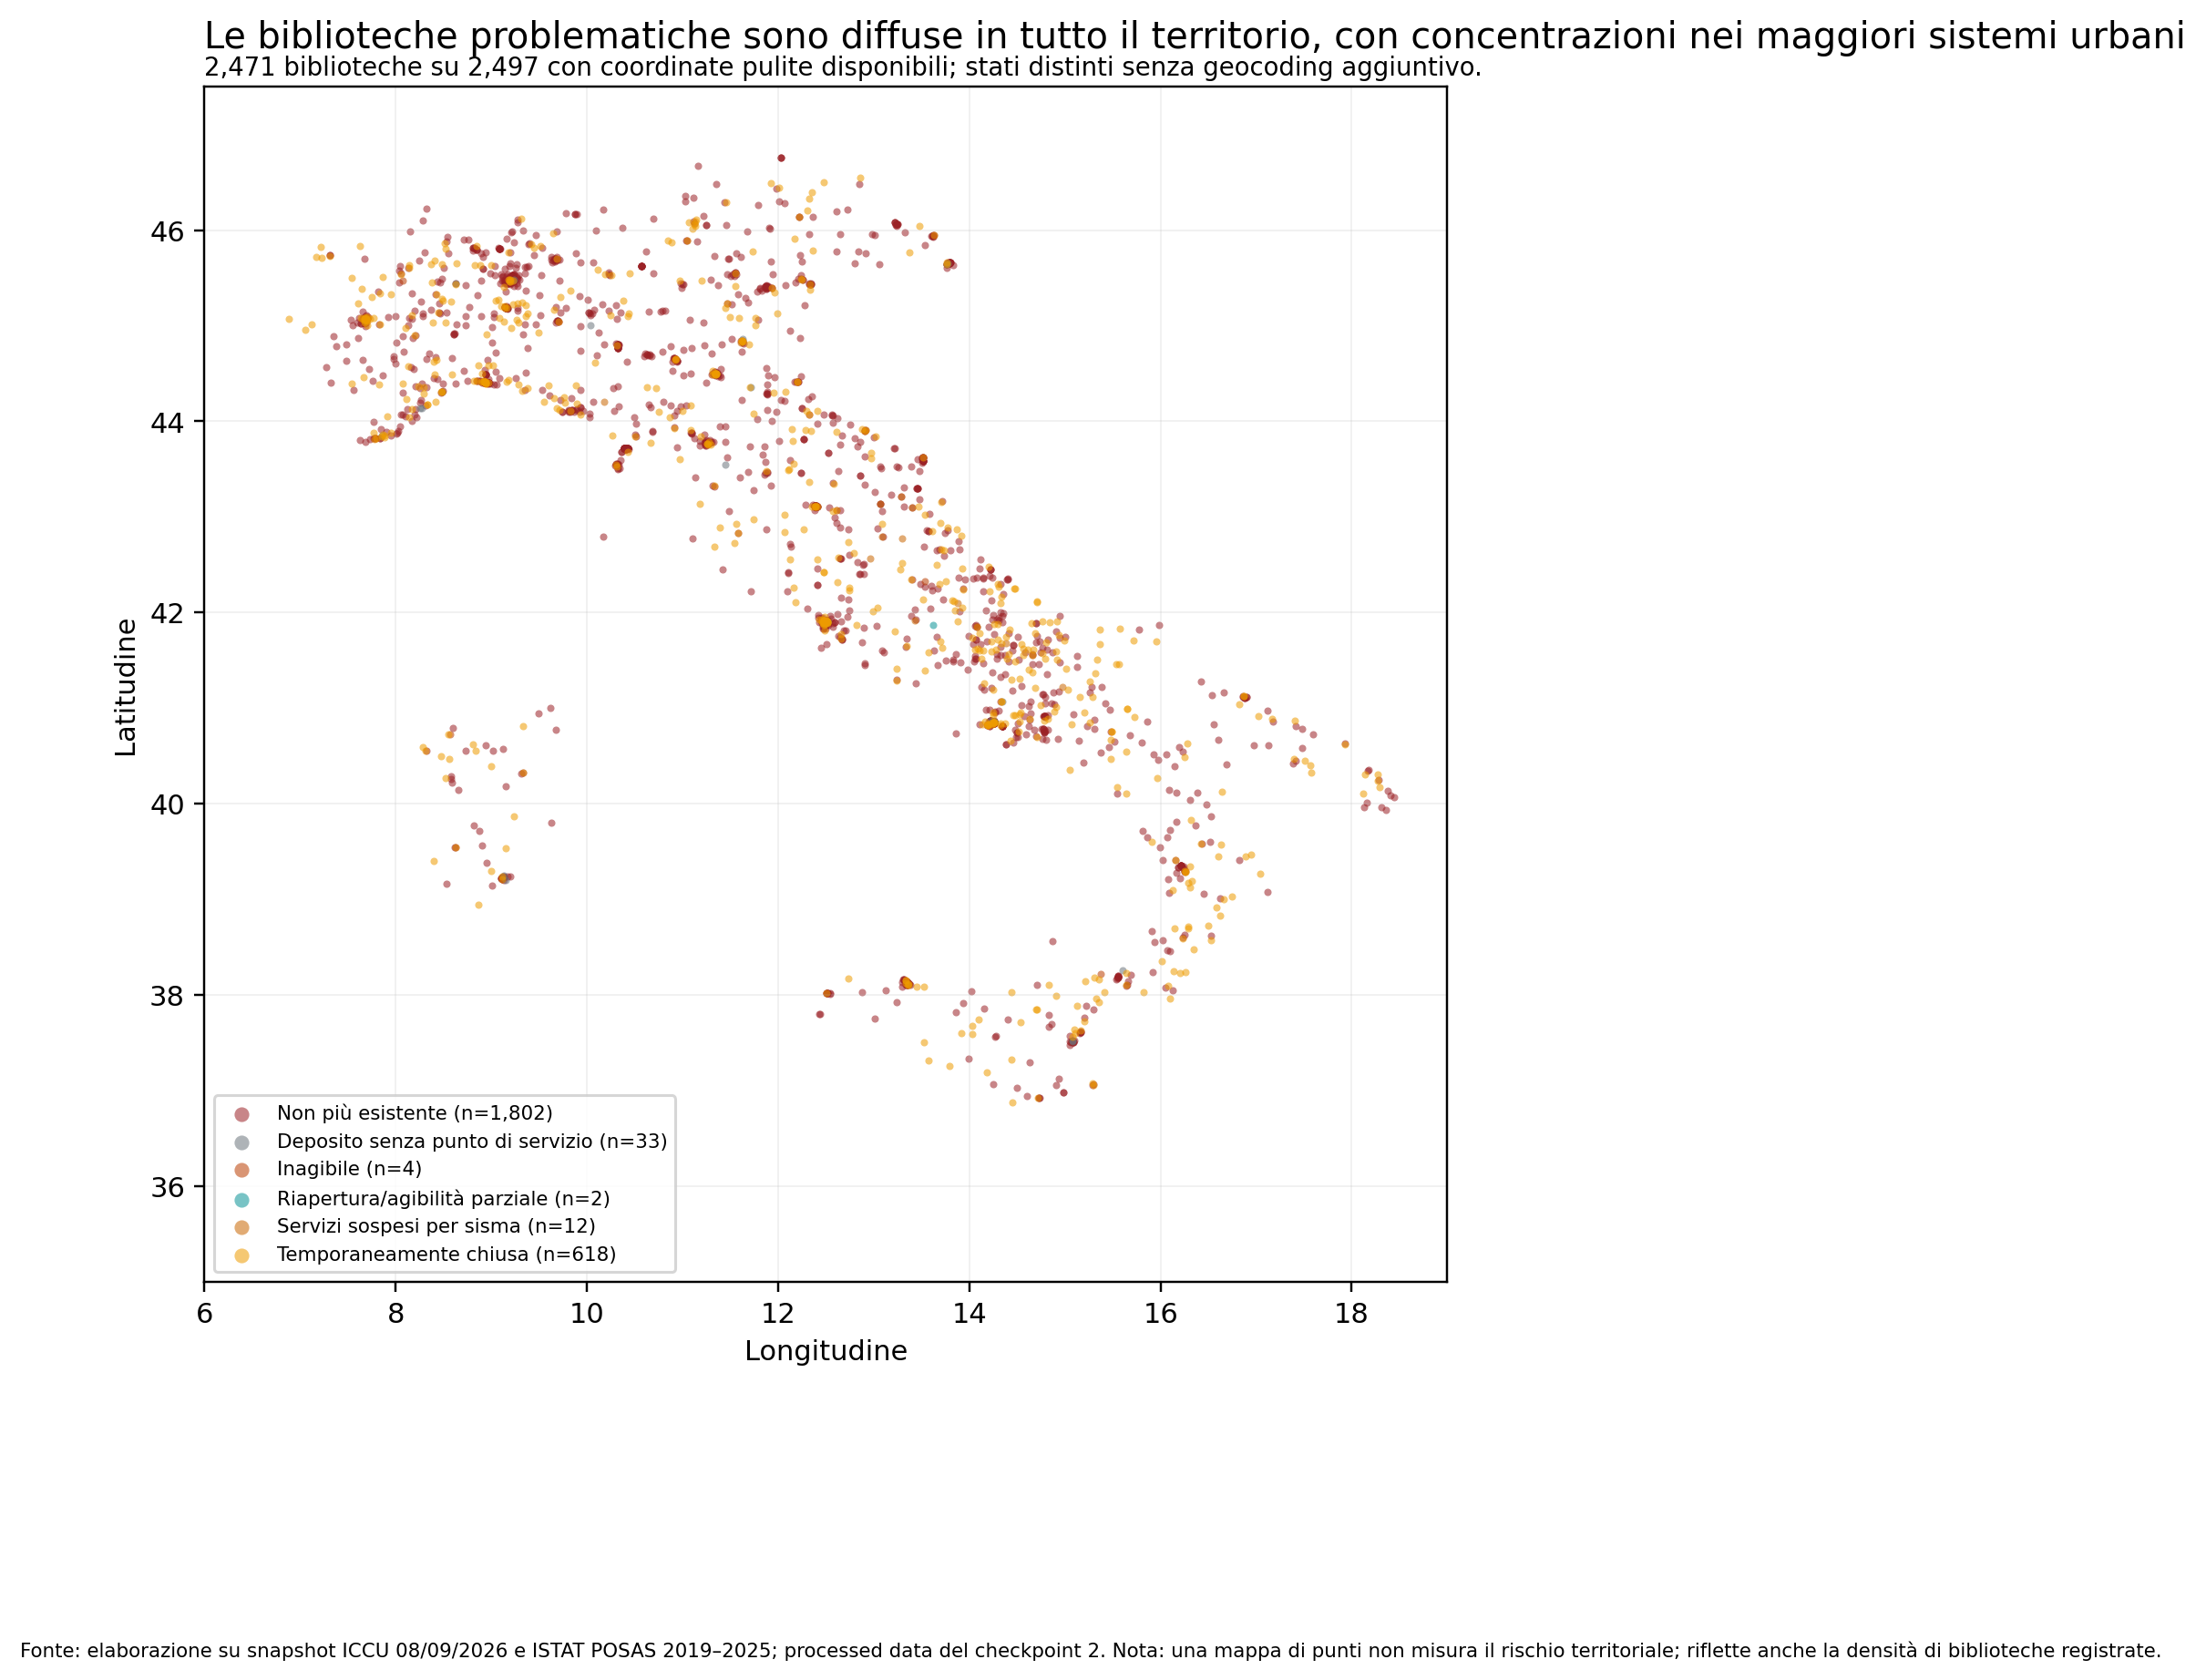
\includegraphics[width=0.79\textwidth]{../visualizations/map_static.png}
\caption{RQ1: mappa statica delle biblioteche problematiche con coordinate pulite.}
\end{figure}

\begin{figure}[H]
\centering
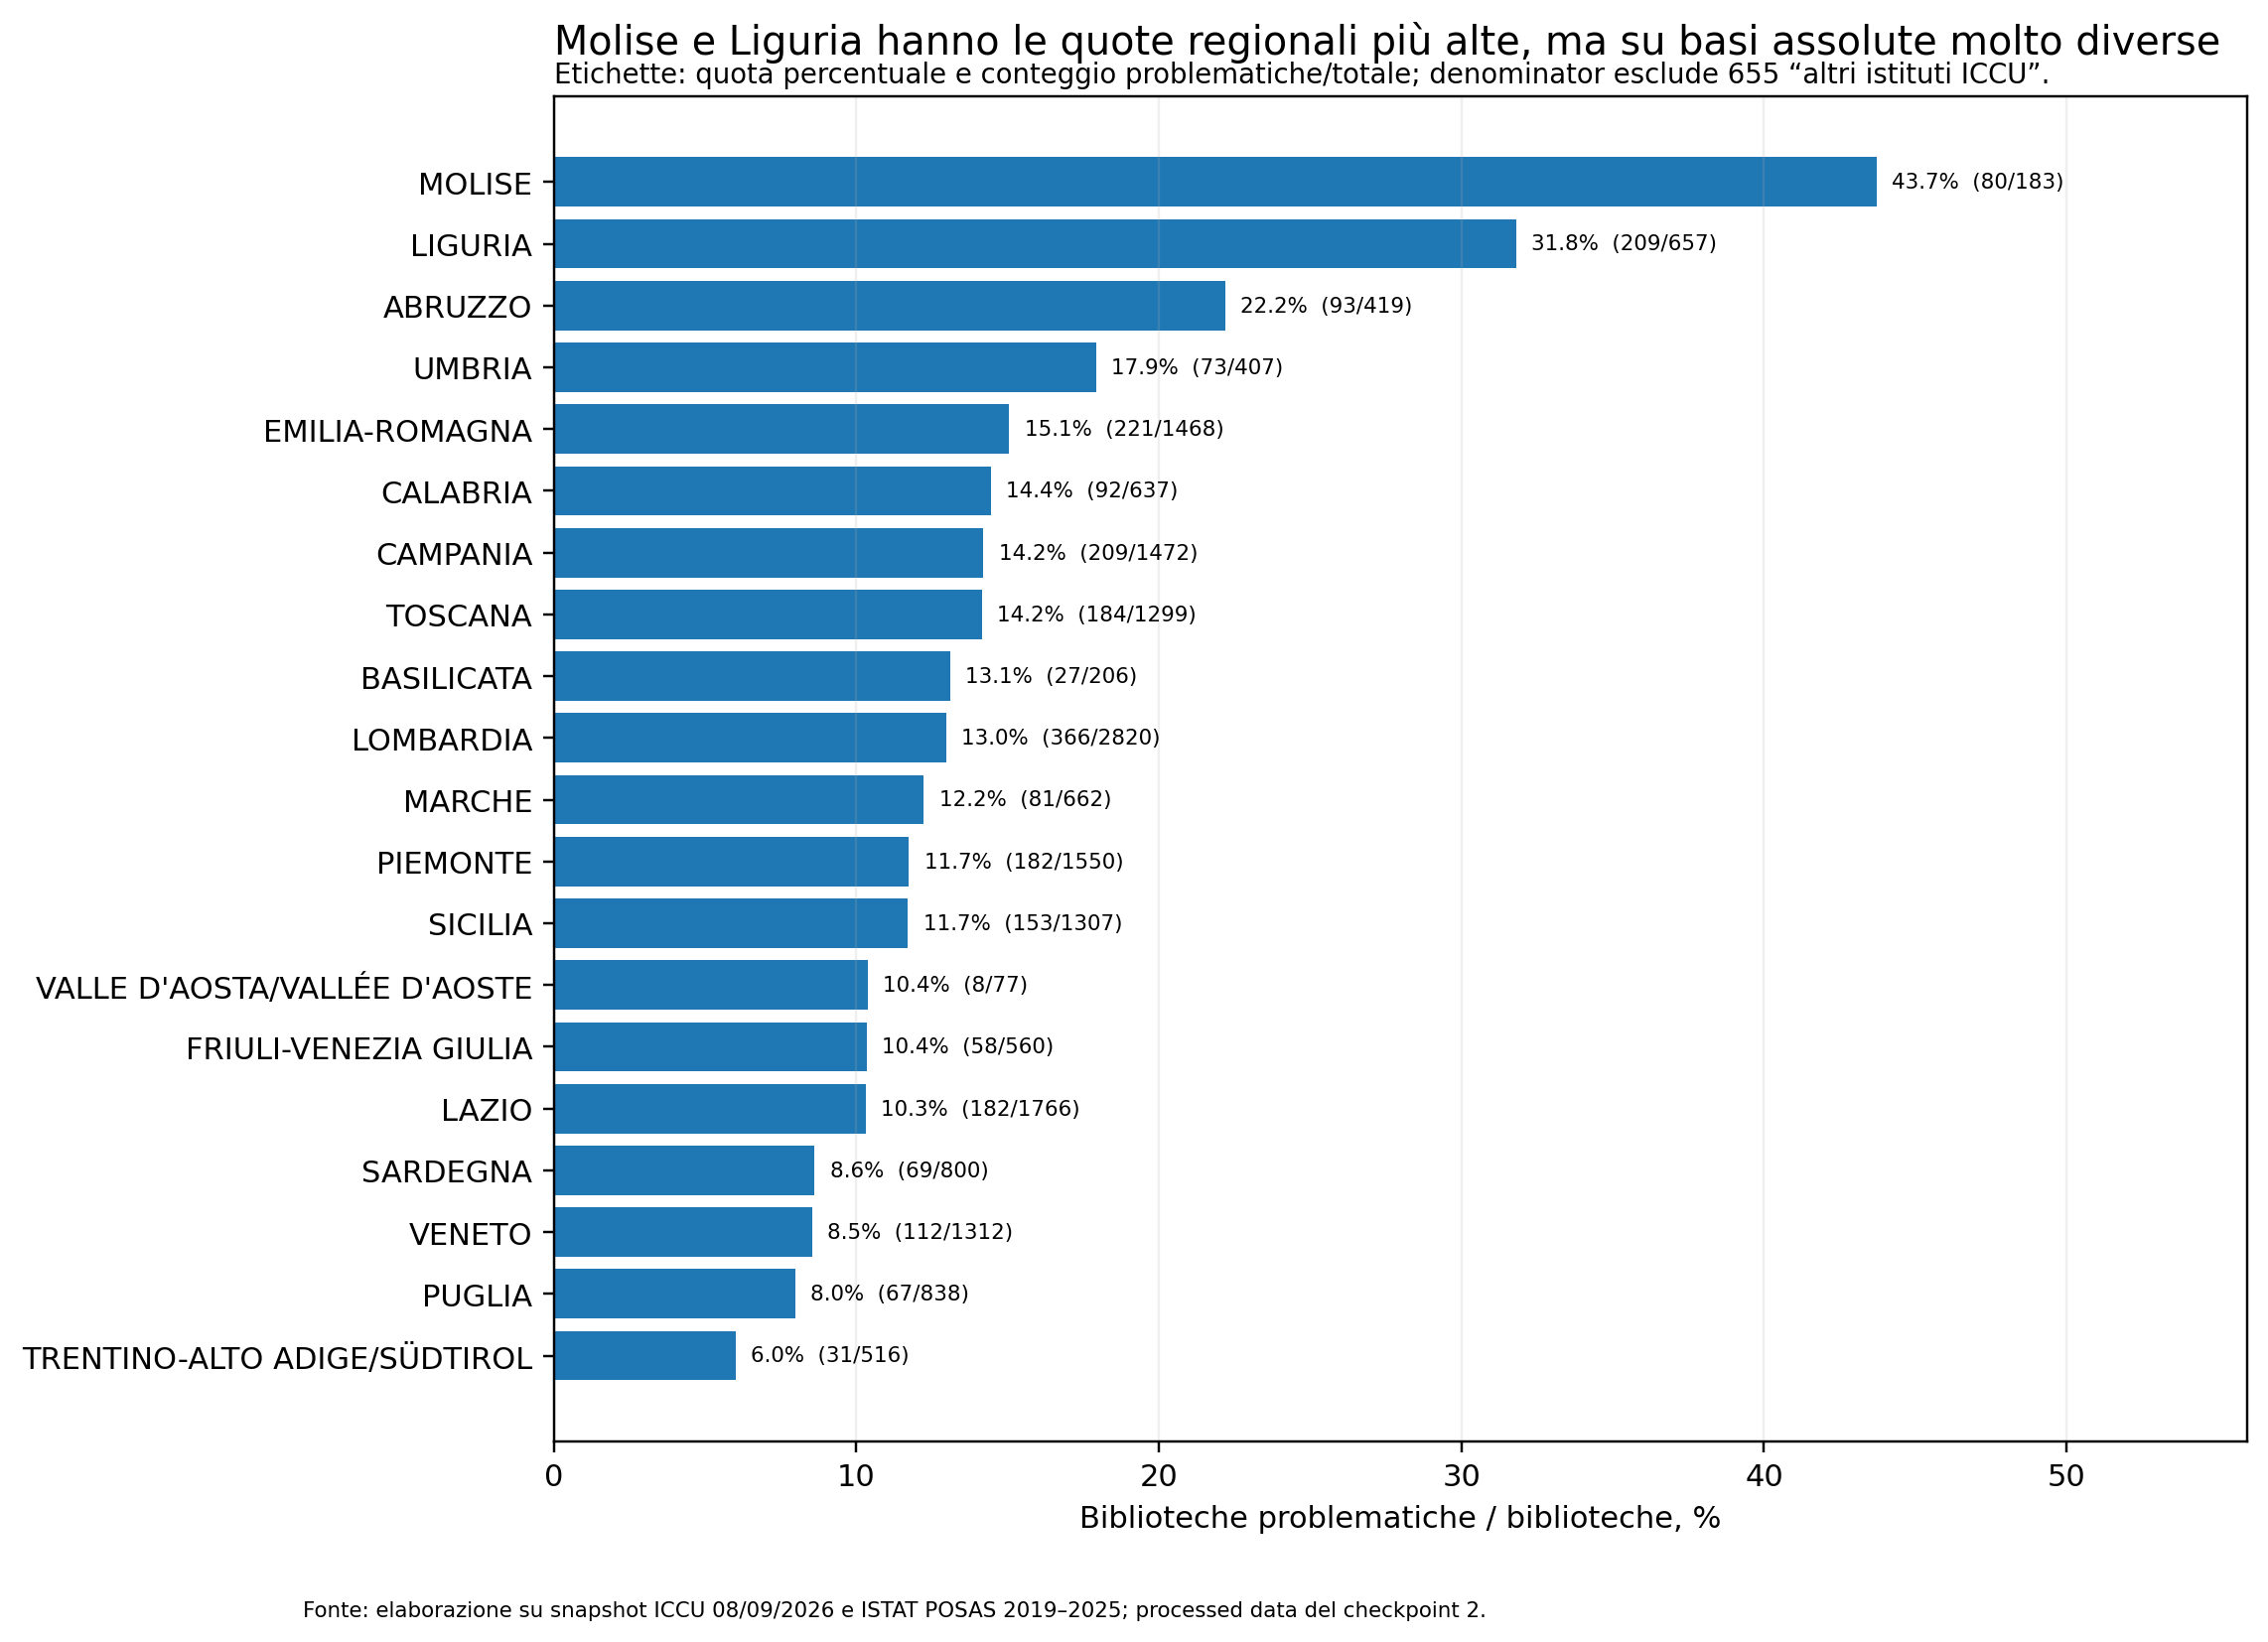
\includegraphics[width=0.98\textwidth]{../visualizations/status_by_region.png}
\caption{RQ1--RQ2: quota regionale con conteggi assoluti annotati.}
\end{figure}

\begin{figure}[H]
\centering
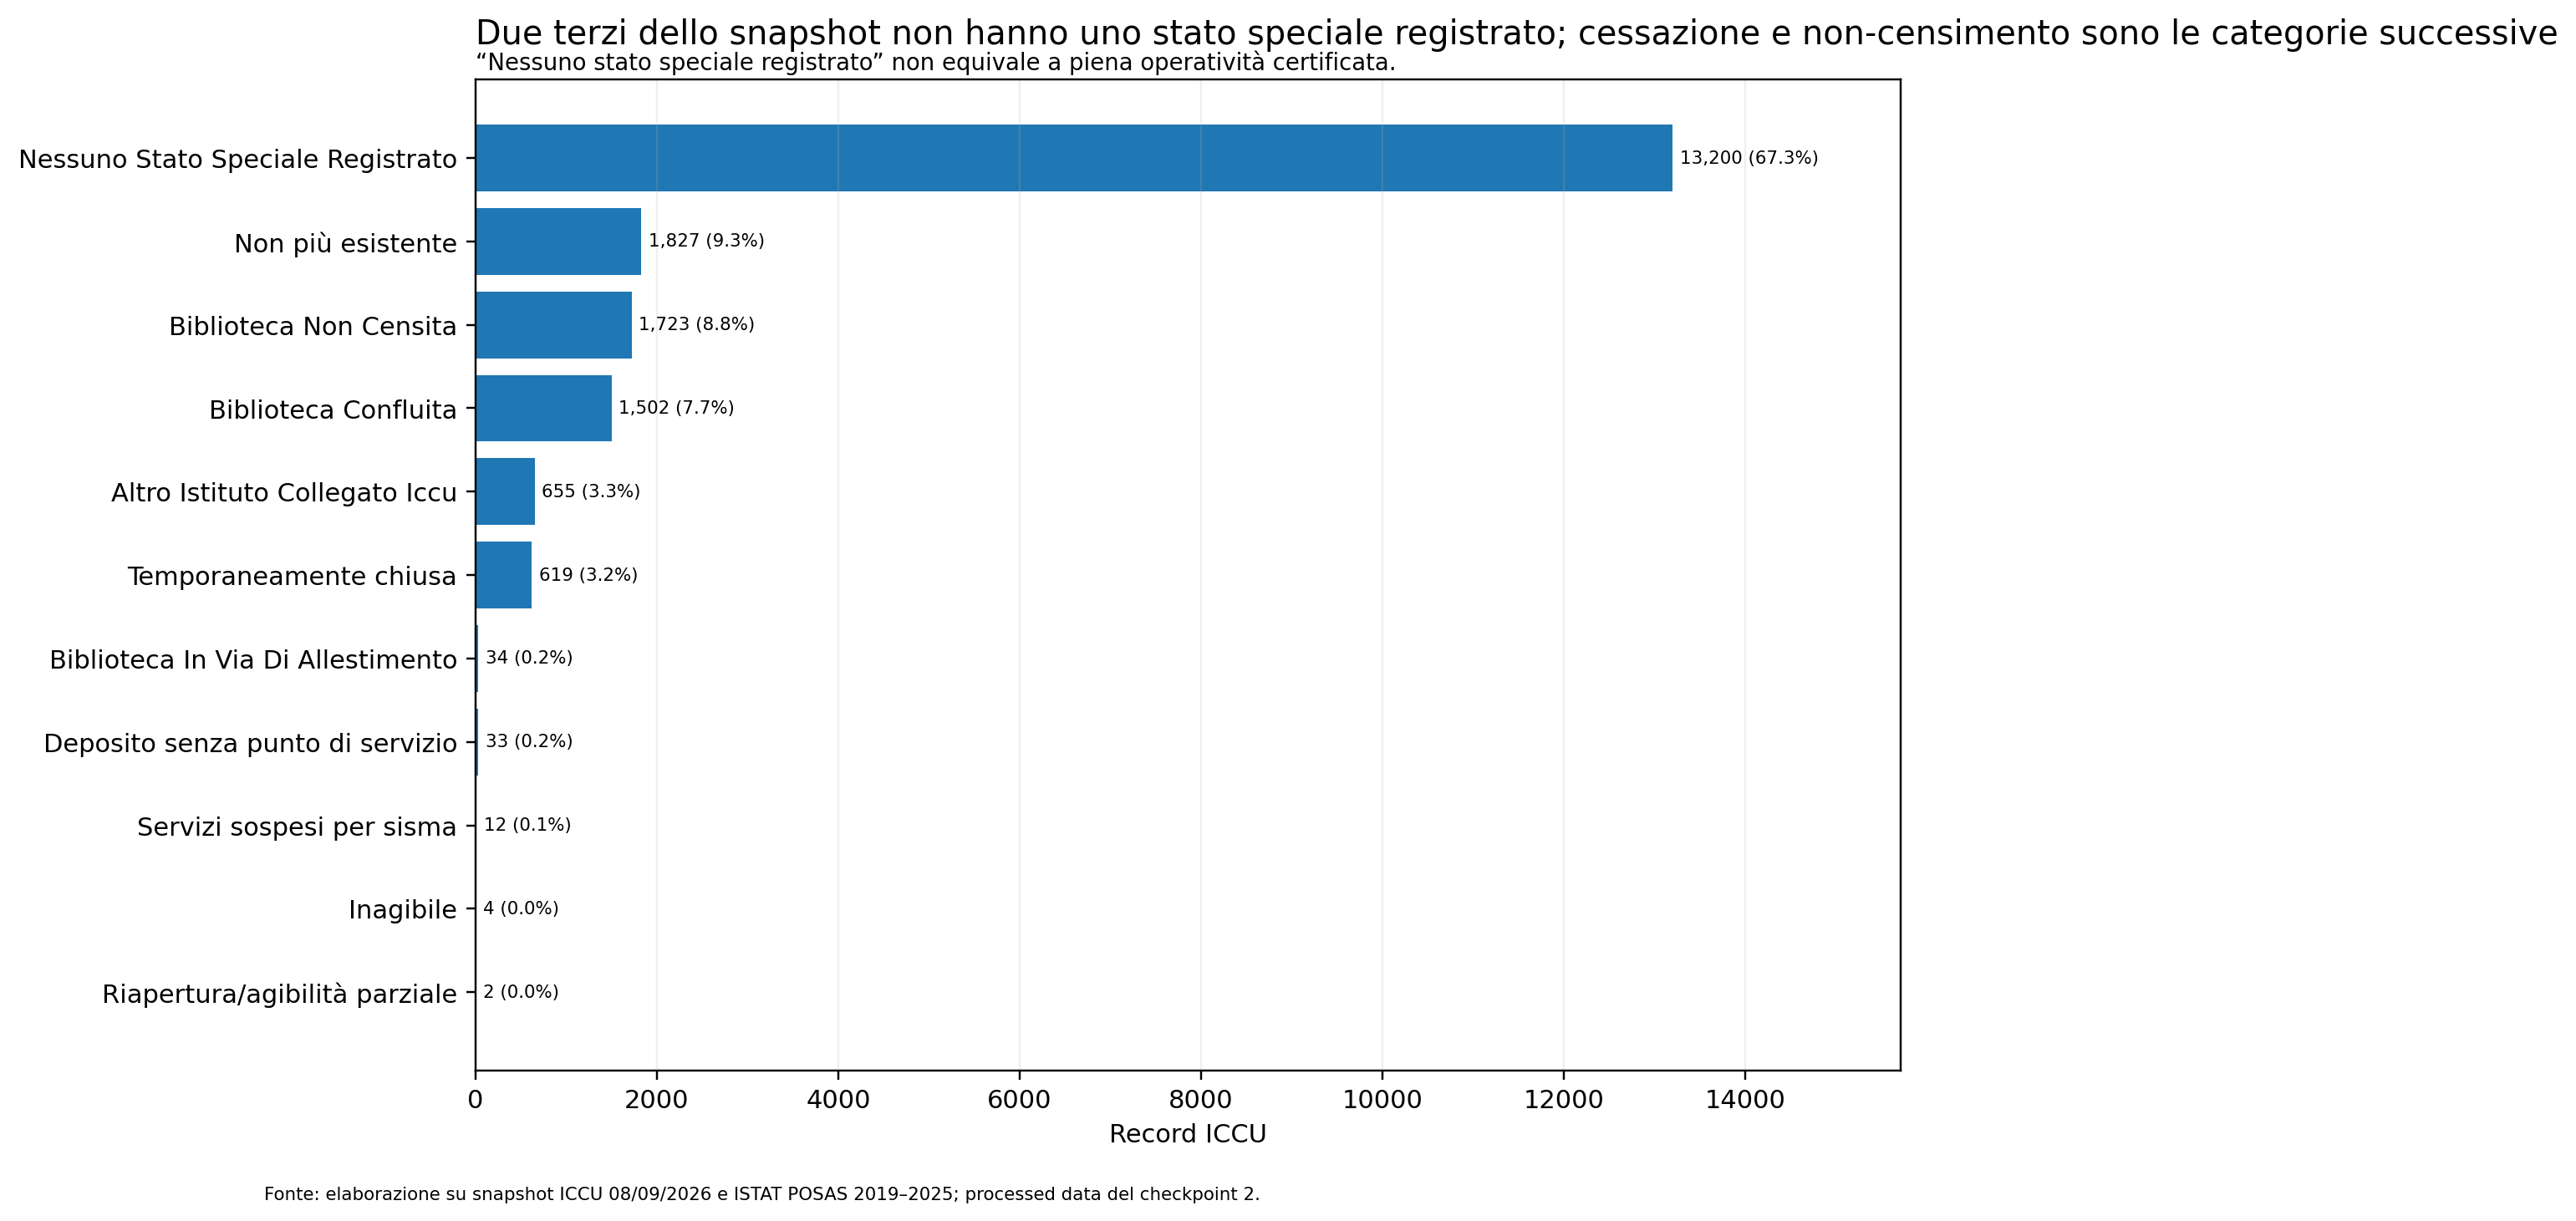
\includegraphics[width=0.94\textwidth]{../visualizations/status_distribution.png}
\caption{RQ2: distribuzione degli stati normalizzati.}
\end{figure}

\begin{figure}[H]
\centering
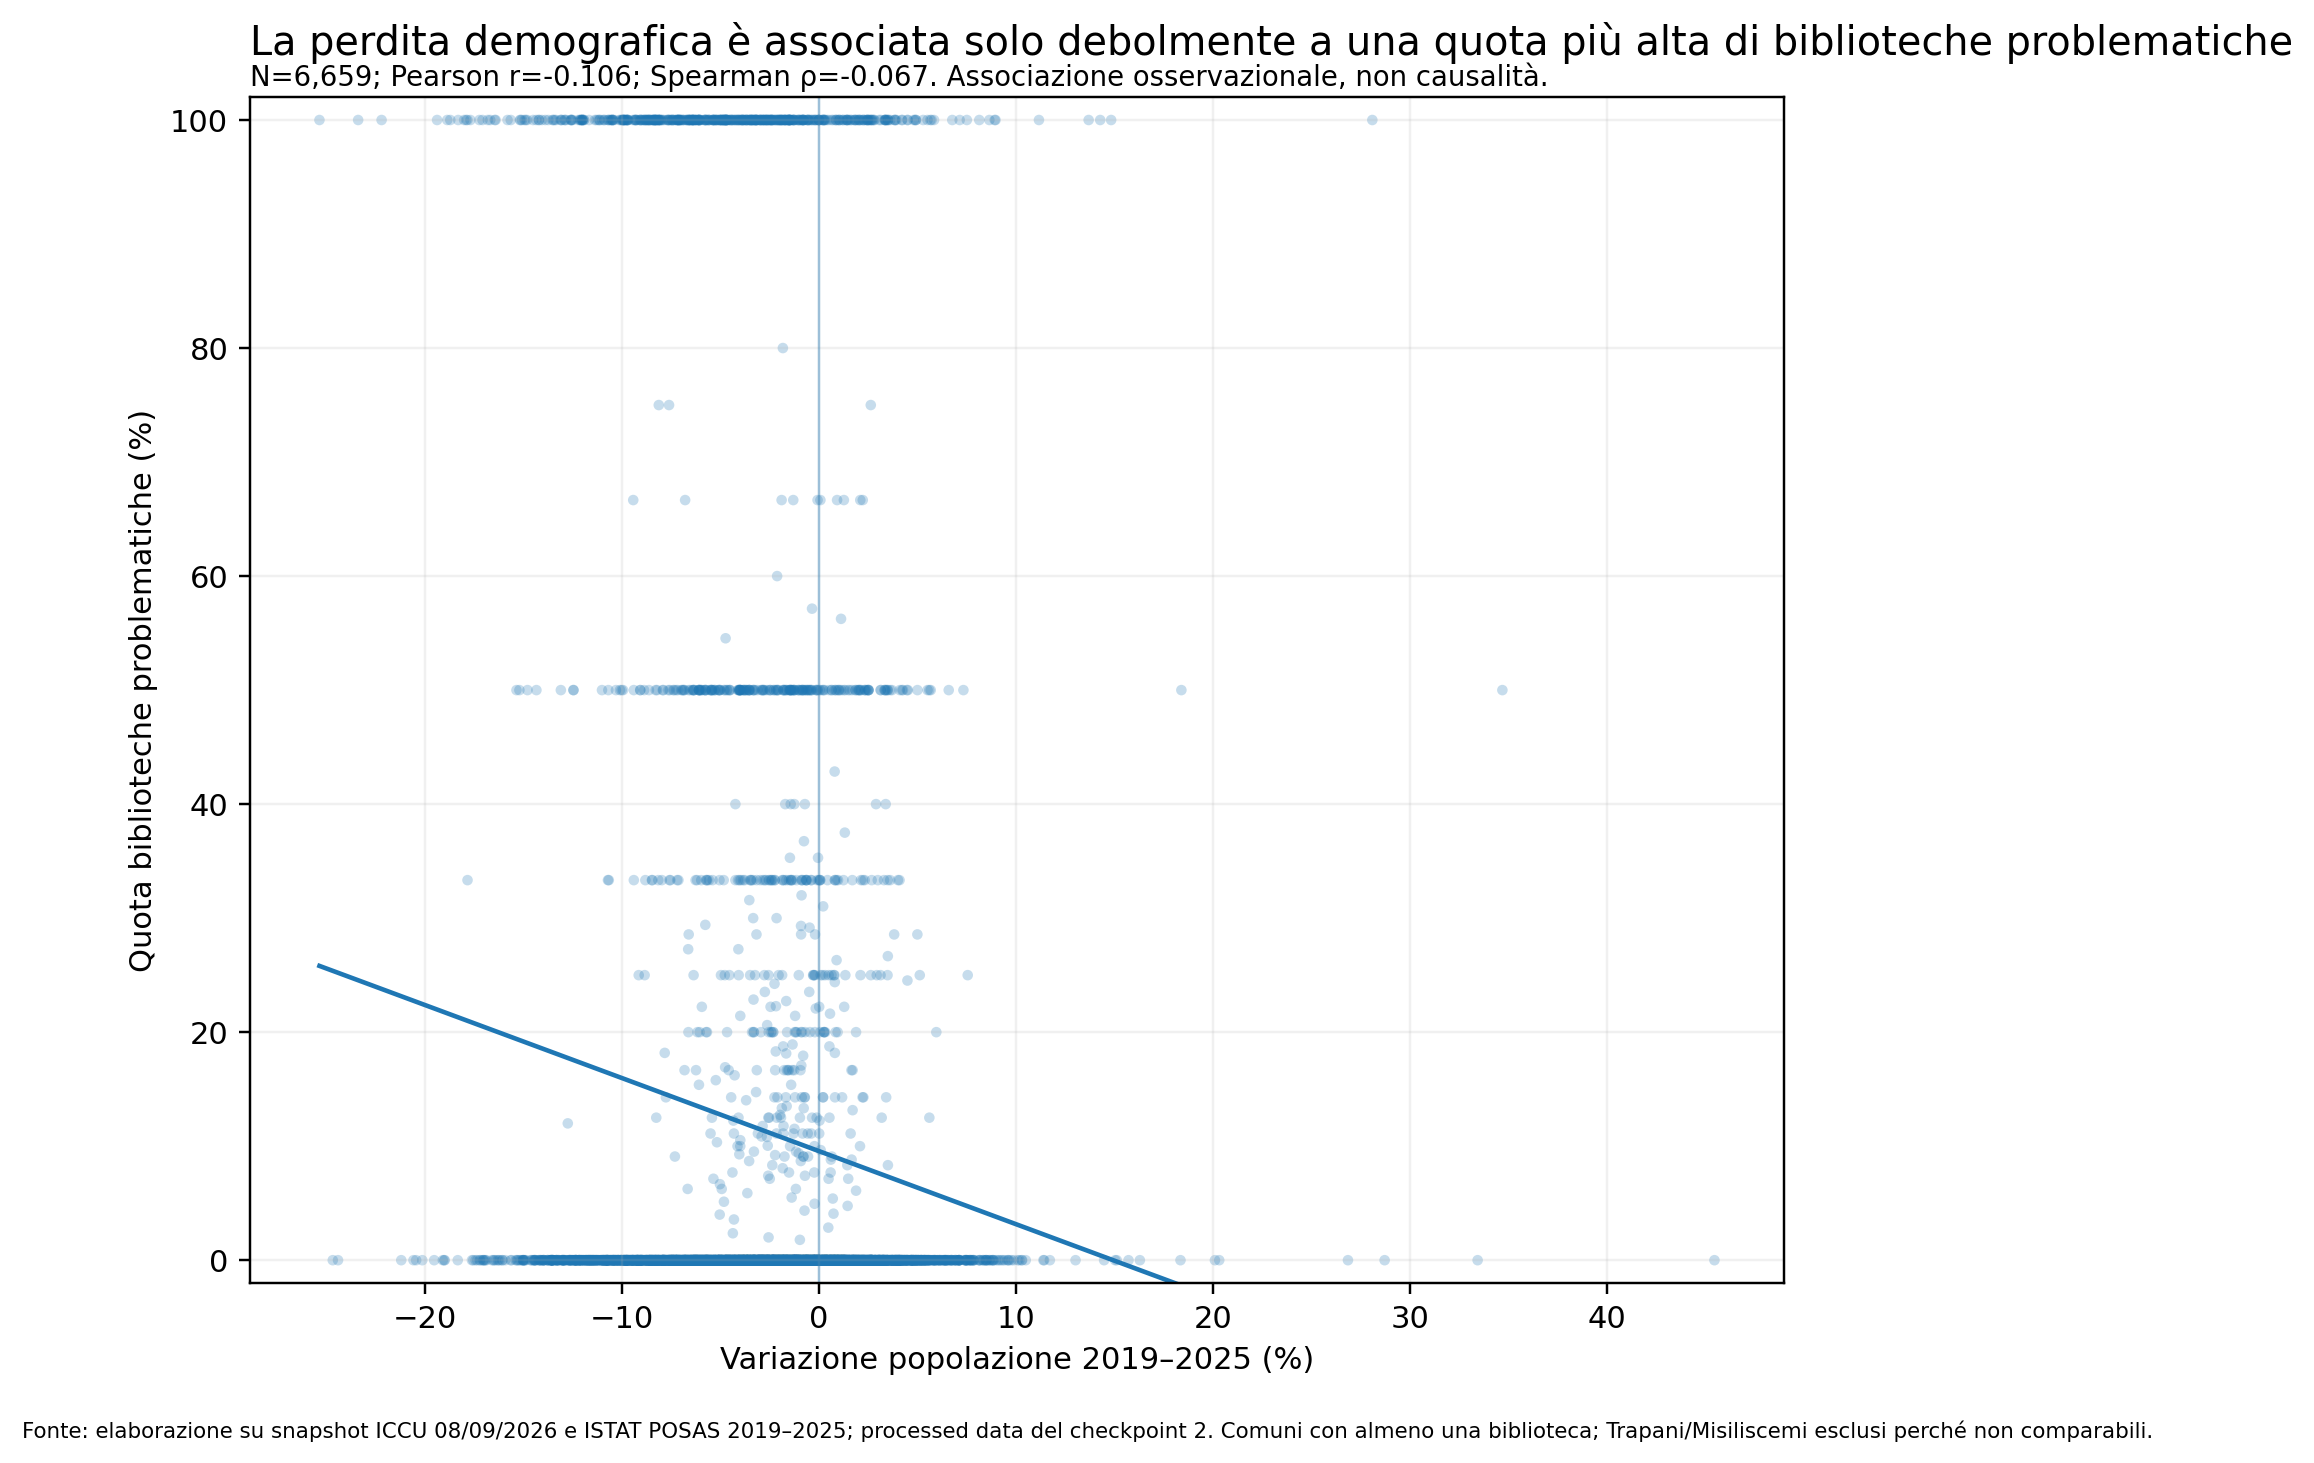
\includegraphics[width=0.88\textwidth]{../visualizations/demography_scatter.png}
\caption{RQ4: variazione demografica 2019--2025 e quota problematica.}
\end{figure}

\begin{figure}[H]
\centering
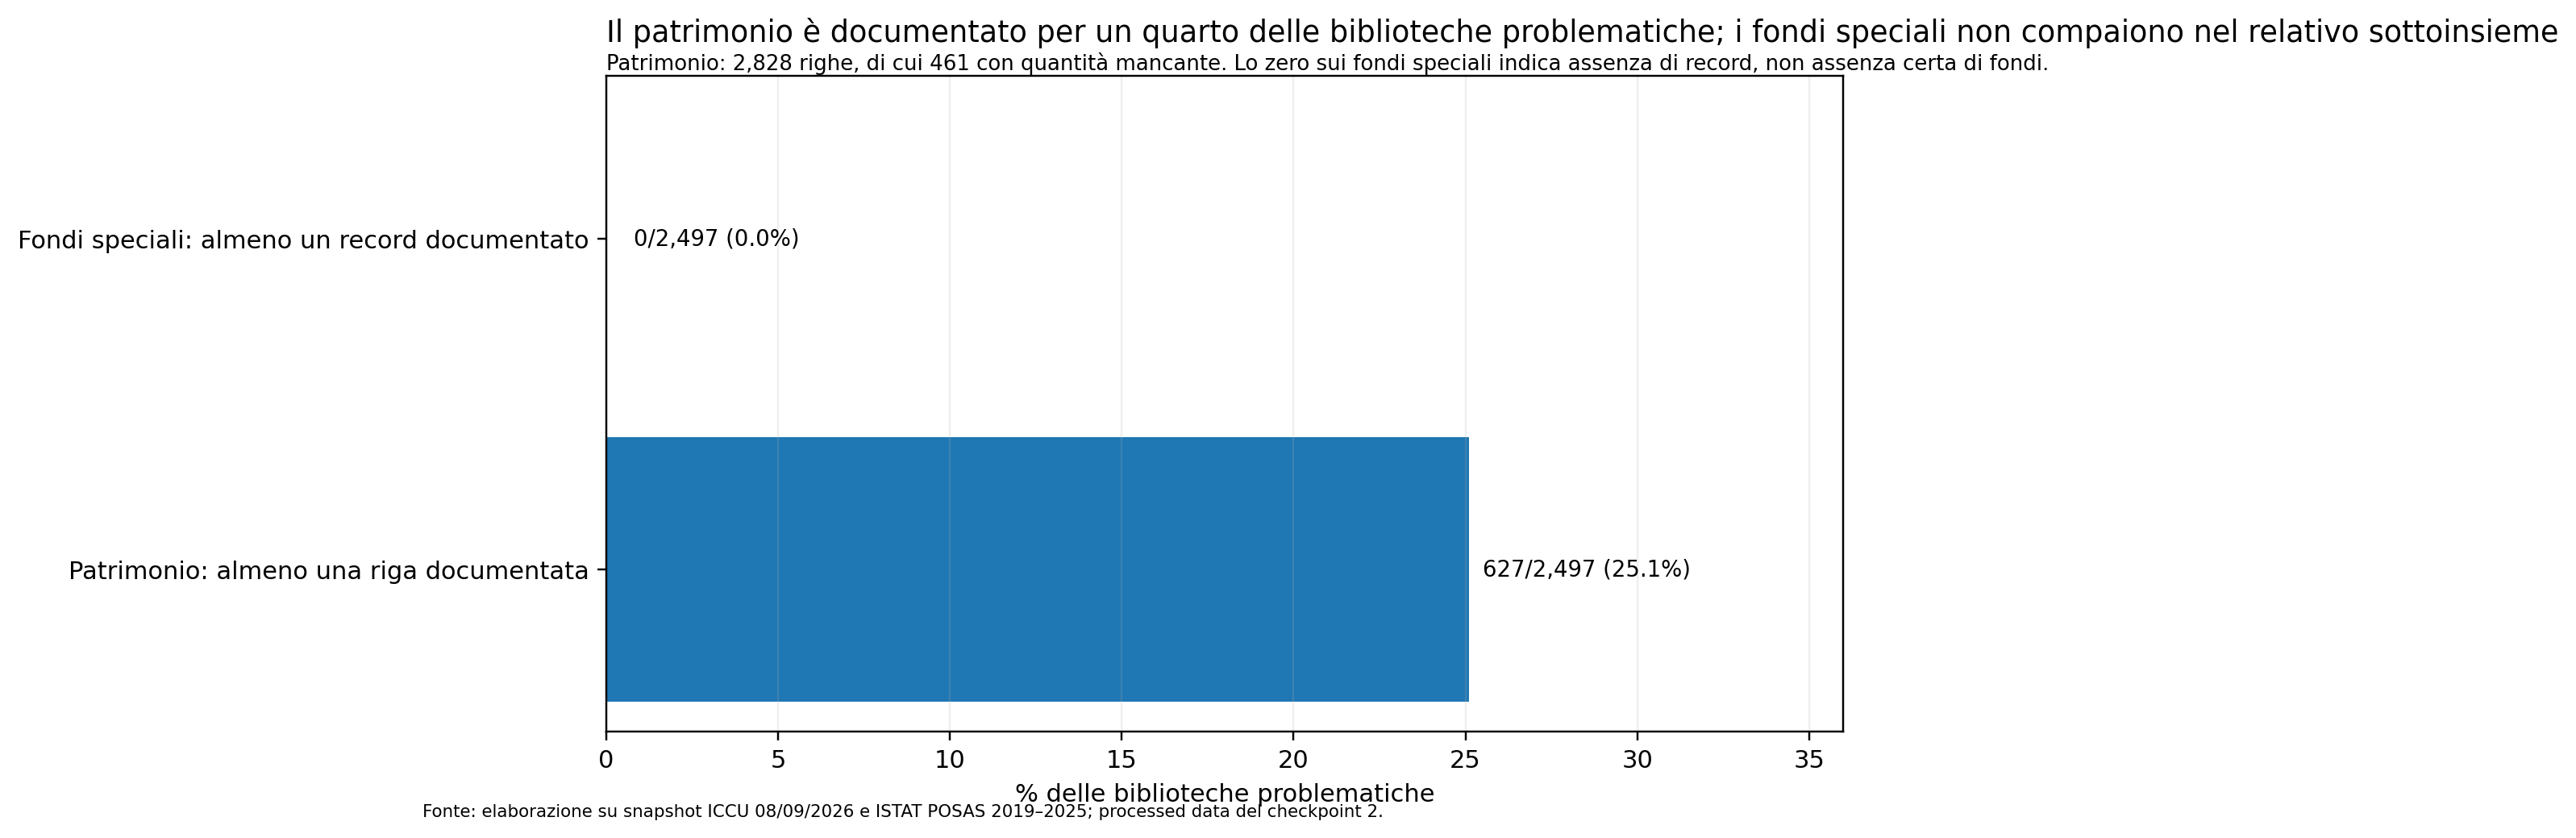
\includegraphics[width=0.92\textwidth]{../visualizations/special_collections.png}
\caption{RQ5: copertura documentaria di patrimonio e fondi speciali nel perimetro problematico.}
\end{figure}

\begin{figure}[H]
\centering
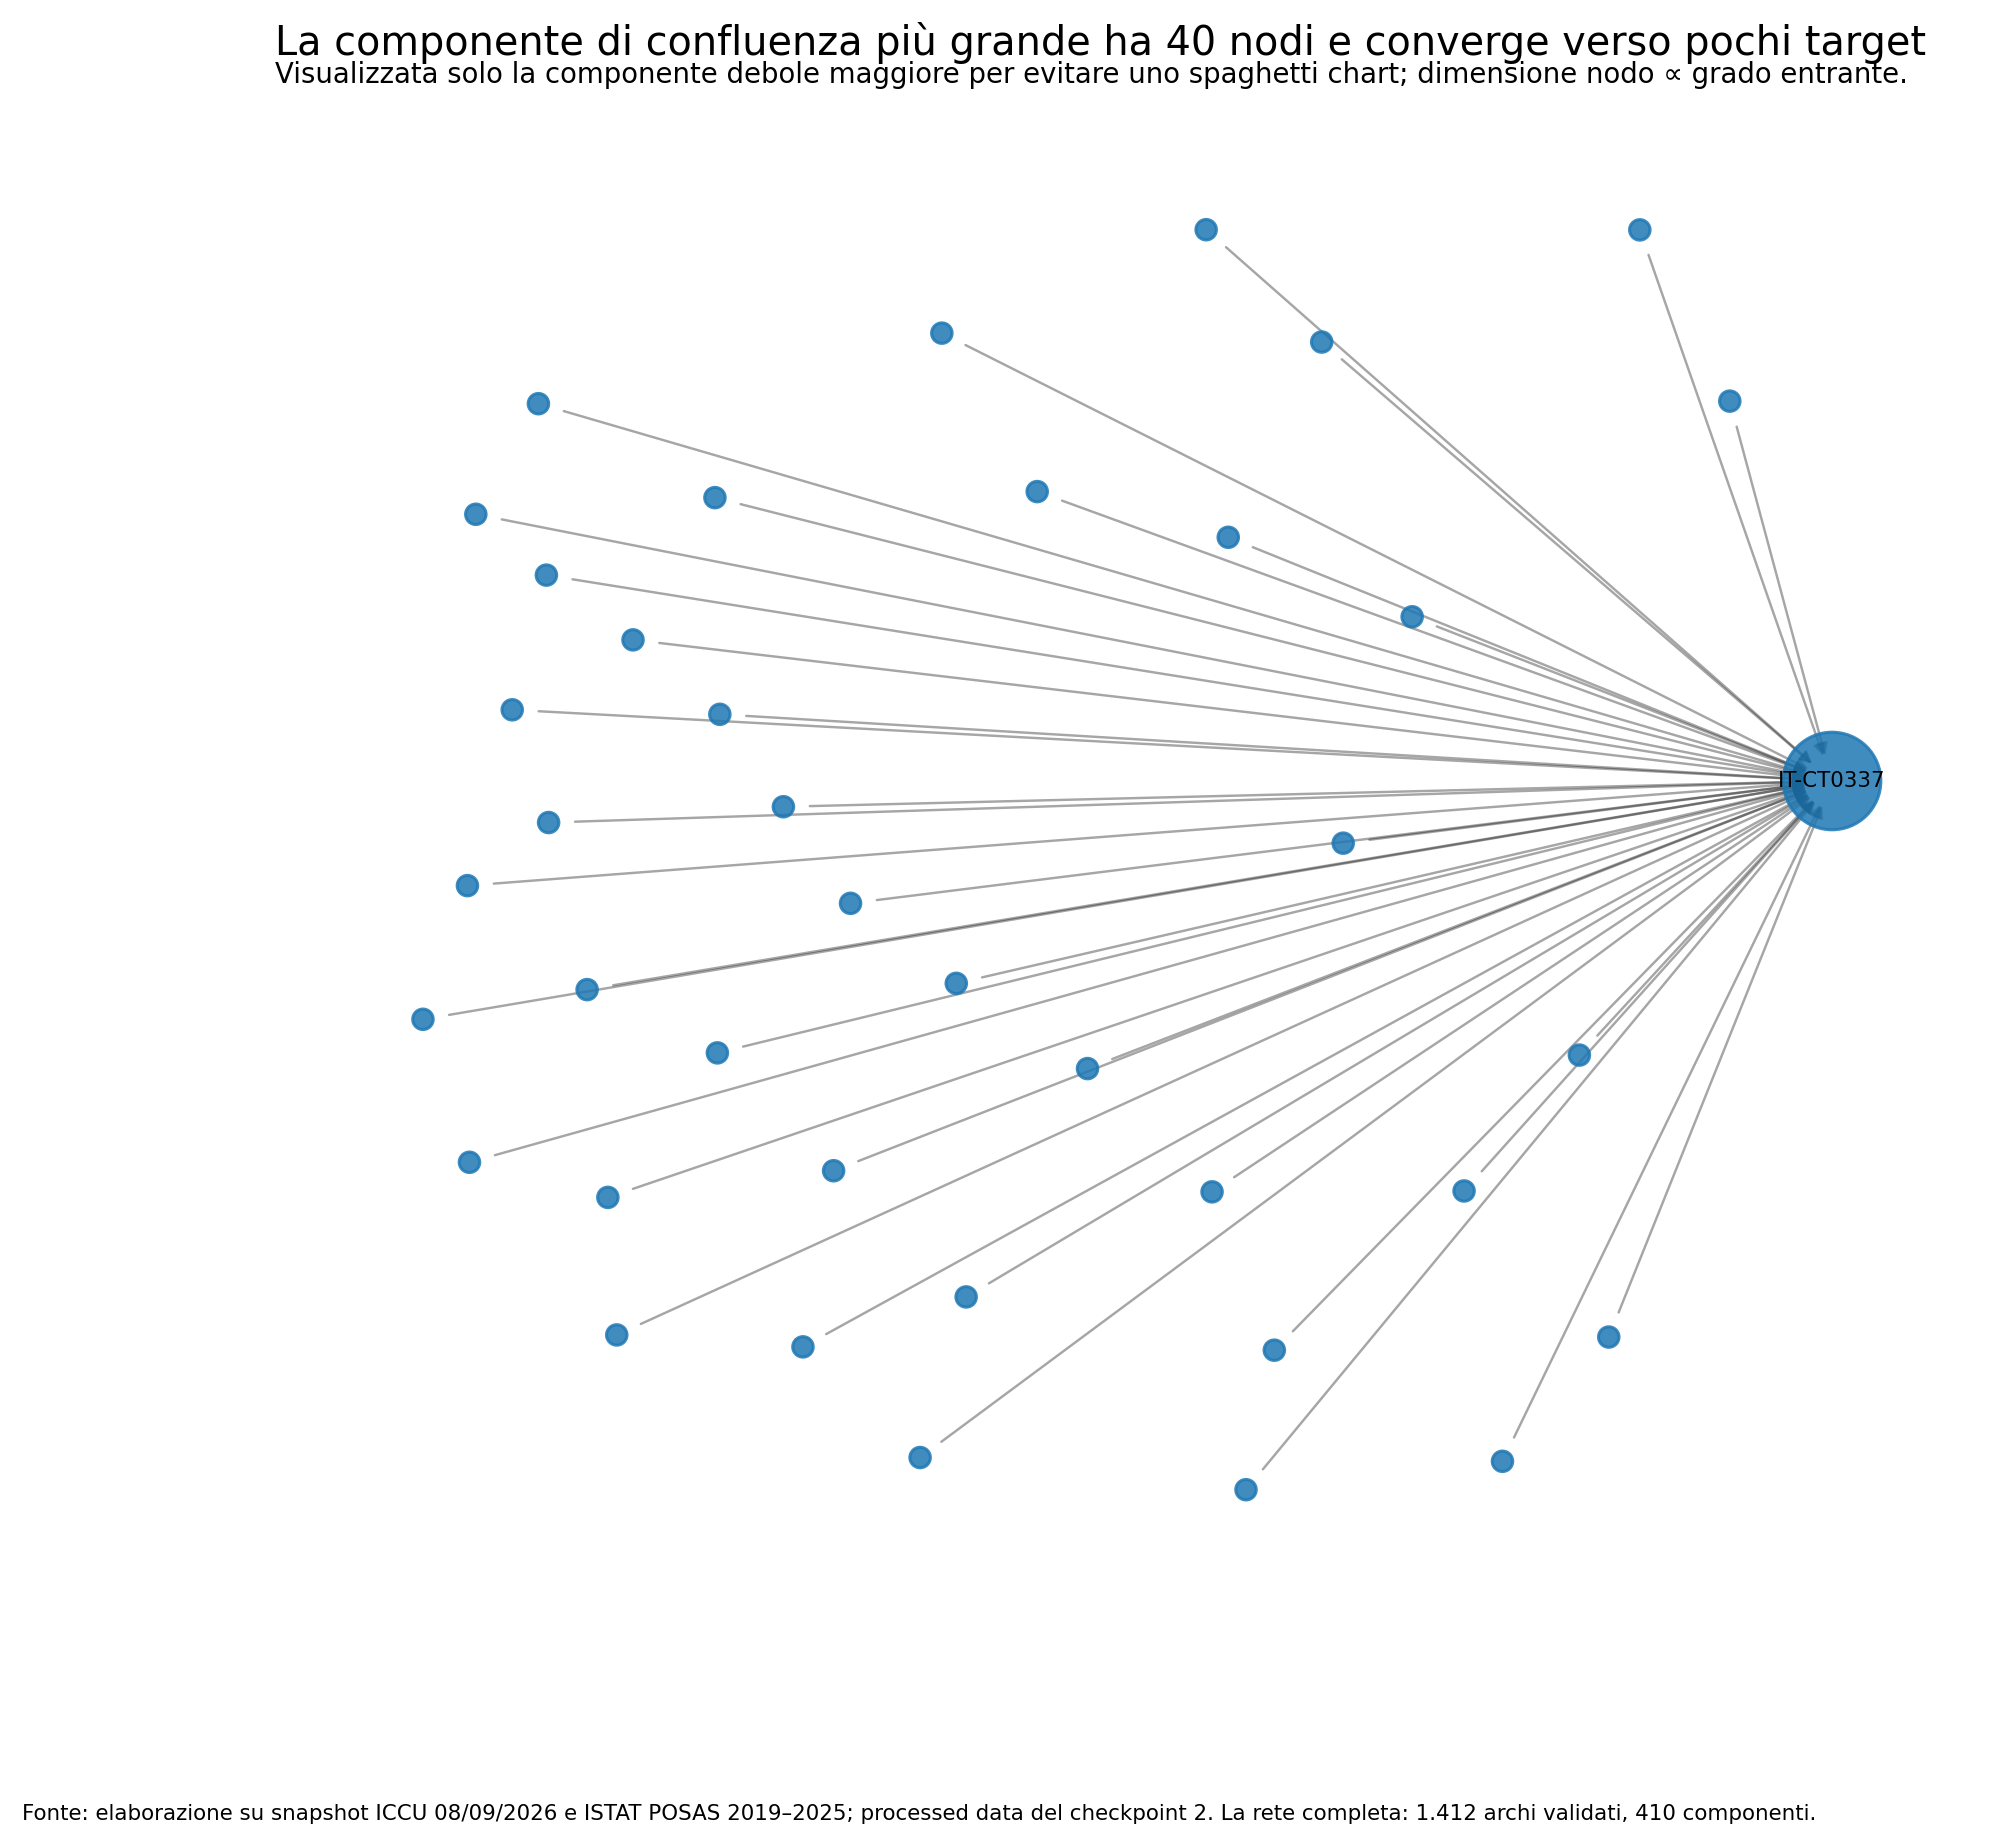
\includegraphics[width=0.86\textwidth]{../visualizations/mergers_network.png}
\caption{RQ7: componente debole maggiore della rete delle confluenze.}
\end{figure}

La versione interattiva della mappa è \texttt{visualizations/library\_map.html}, con clustering e layer per stato. Le figure statiche sono esportate ad alta risoluzione e includono fonte e note metodologiche.

\section{Problemi e decisioni progettuali}
Il \texttt{decisions\_log.md} registra le decisioni nel formato problema--evidenza--alternative--decisione--motivazione--conseguenza. Tra le scelte più rilevanti: preservare relazioni 1:N; distinguere stati ICCU; usare una geografia 2025; non imputare missing; riusare coordinate ICCU senza geocoding; separare analisi tabellare da SPARQL; usare URI \texttt{.invalid} finché non esiste un dominio; visualizzare solo la componente maggiore della rete.

Durante la Fase 3 non sono emerse discrepanze che richiedessero la rigenerazione di ontologia, RDF o interlinking. È emerso invece un limite dell'ambiente: nessun motore Parquet installato e impossibilità di installare \texttt{pyarrow} senza rete. Invece di creare file falsi, il repository conserva i CSV e fornisce \texttt{scripts/export\_parquet.py} come operazione riproducibile residua.

\section{Limiti}
\begin{enumerate}
\item Lo snapshot ICCU non rappresenta necessariamente una serie storica completa.
\item Lo stato osservato non fornisce automaticamente data di inizio o fine.
\item ``Nessuno stato speciale registrato'' non certifica piena operatività.
\item La completezza ICCU varia tra biblioteche e dataset secondari.
\item Patrimonio mancante non equivale a patrimonio inesistente.
\item Fondo speciale non documentato non equivale ad assenza del fondo.
\item La correlazione demografica non dimostra causalità.
\item Fusioni, incorporazioni e scorpori comunali complicano i confronti 2019--2025.
\item URI ed endpoint esterni possono cambiare o diventare indisponibili.
\item ``Biblioteche Fantasma'' è un'etichetta narrativa e non una categoria ufficiale ICCU.
\item Il denominatore delle quote regionali esclude i 655 record classificati come altri istituti collegati ICCU; usare il totale del registro produrrebbe un indicatore diverso.
\item Il dataset delle tipologie copre 13.715 biblioteche, perciò RQ3 non descrive con la stessa completezza l'intero master.
\item La quota problematica comunale è discreta e fortemente influenzata dai comuni con poche biblioteche: una singola osservazione può produrre quote pari a 0 o 100\%.
\item La somma delle quantità patrimoniali note può includere livelli di aggregazione non omogenei (materiali specifici e ``totale posseduto'') e non è un inventario additivo complessivo.
\item La rete delle confluenze deriva dallo stato osservato nello snapshot e non contiene necessariamente tutte le trasformazioni storiche.
\item GraphDB non è stato eseguito; SHACL è validato nel sottoinsieme Core implementato; l'esecuzione SPARQL è parziale.
\item Le URI locali non sono dereferenziabili e impediscono una dichiarazione operativa di 5-star Linked Open Data.
\item Gli archivi RAW non sono contenuti nel checkpoint finale; sono conservati hash e provenance, ma una riproduzione end-to-end della Fase 1 richiede le sorgenti esterne originali.
\item I Parquet non sono stati materializzati nell'ambiente di build per assenza di un engine disponibile offline.
\end{enumerate}

\section{Conclusioni}
Il progetto dimostra l'intero percorso logico dagli Open Data tabellari a un knowledge graph interlinkato, mantenendo separati dati, semantica e interpretazione. Le 2.497 biblioteche del perimetro problematico rappresentano il 13,17\% delle 18.956 biblioteche del denominatore analitico. La distribuzione territoriale è molto eterogenea: le quote più alte sono in Molise e Liguria, mentre i maggiori valori assoluti si osservano nei sistemi bibliotecari più grandi, come Lombardia e grandi città.

RQ4 non supporta una narrazione forte secondo cui lo spopolamento ``spiega'' le biblioteche problematiche: la relazione è negativa ma debole. Questo risultato è metodologicamente utile proprio perché impedisce una data story causale non supportata. RQ5 evidenzia un altro aspetto centrale: la copertura dei dati secondari. È possibile descrivere il patrimonio documentato per 627 biblioteche problematiche, ma l'assenza di fondi speciali nel sottoinsieme è una mancanza di record, non una prova di assenza reale.

La rete delle confluenze mostra una struttura frammentata con numerosi piccoli componenti e alcuni hub di destinazione. Sul versante Linked Data, l'interlinking è molto elevato grazie a identificatori ufficiali: 100\% per le biblioteche e 99,9620\% per i comuni. Resta tuttavia un confine netto tra un grafo \emph{predisposto} al Web of Data e una pubblicazione 5-star effettiva: senza dominio pubblico e URI dereferenziabili, il livello massimo non può essere dichiarato operativo.

In termini didattici, il valore del progetto non è la dimensione del grafo ma la tracciabilità tra Research Question, dato, metodo, risultato, visualizzazione, interpretazione e limite. Le scelte conservative sui missing, sugli stati, sulle equivalenze esterne e sulla causalità sono parte integrante della qualità del risultato.

\section{Fonti e riferimenti}
\printbibliography[heading=none]

\end{document}
